
\chapter{Experimental Setup}\label{sec:experimentalsetup}

In the experiment performed at ETH Oct. 11th, 2012 an axial fan LTG is used, powered by a 7kW electrical engine providing up to 5000 rpm. The experimental setup consists of a 3m long inlet tunnel and a diffuser behind the probe device (Figure \ref{fig:f2}). 

\begin{figure}[H]
\centering
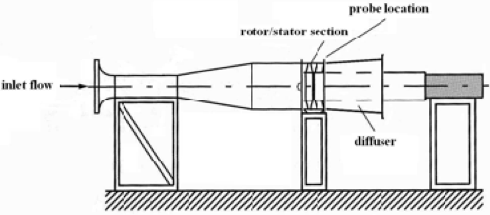
\includegraphics[width=0.5\textwidth]{pics/f2.png}
\caption{Overview Test Rig LTG}
\label{fig:f2}
\end{figure}

The actual fan comprises a rotor (upstream) and a stator behind. The probe is located downstream of the stator and can be moved in radial, circumferential $(\Theta)$ and yaw $(\gamma)$ direction. The cobra shaped five-hole probe (Figure \ref{fig:f3} measures the individual pressures of the holes $(\o~ 2mm)$. 

\begin{figure}[H]
\centering
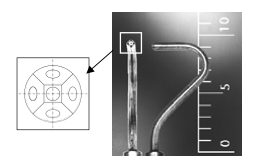
\includegraphics[width=0.3\textwidth]{pics/f3.png}
\caption{Cobra-Shaped 5-Hole Probe}
\label{fig:f3}
\end{figure}

With this data yaw angle, pitch angle, total pressure, static pressure and Mach number are computed. Now absolute velocity and its components can be derived.


